\begin{mlproblem}[V for Voronoi]{5+5=10}
Recall the learning with prototypes problem. Consider a two class problem where the prototypes are the points $(1,0)$ (green) and $(0,1)$ (red). Calculate the decision boundary when we use the learning with prototypes rule but with the following \emph{Mahalanobis} metrics. In the following, $\vz^1,\vz^2 \in \bR^2$ denote two points on the real plane
\begin{enumerate}
	\item $d(\vz^1,\vz^2) = \ip{\vz^1-\vz^2}{U(\vz^1-\vz^2)}$, where $U = \bs{\begin{array}{cc}
		3&0\\0&1
	\end{array}}$
	\item $d(\vz^1,\vz^2) = \ip{\vz^1-\vz^2}{V(\vz^1-\vz^2)}$, where $V = \bs{\begin{array}{cc}
		1&0\\0&0
	\end{array}}$
\end{enumerate}
Figure~\ref{fig:proto} pictorally depicts the prototypes as well as the sample solution if we had used the standard Euclidean metric to compute distances. In your submission, for each of the two parts above, you must include the following details
\begin{enumerate}
	\item The mathematical expression for the decision boundary. For example, in the Euclidean case, it is the line $y = x$.
	\item An image shading the red and green decision boundaries for the above cases similar to the figure on the right in Figure~\ref{fig:proto}.
\end{enumerate}
To aid you, both figures in Figure~\ref{fig:proto} have been included in your assignment package (\verb|proto_blank.png| and \verb|proto_euclid_sample.png|). Note that your images must be embedded in your PDF file and not sent separately. Use the \verb!\includegraphics! command in \LaTeX{} to embed images in your submission PDF file.
\begin{figure}[th]%
\centering
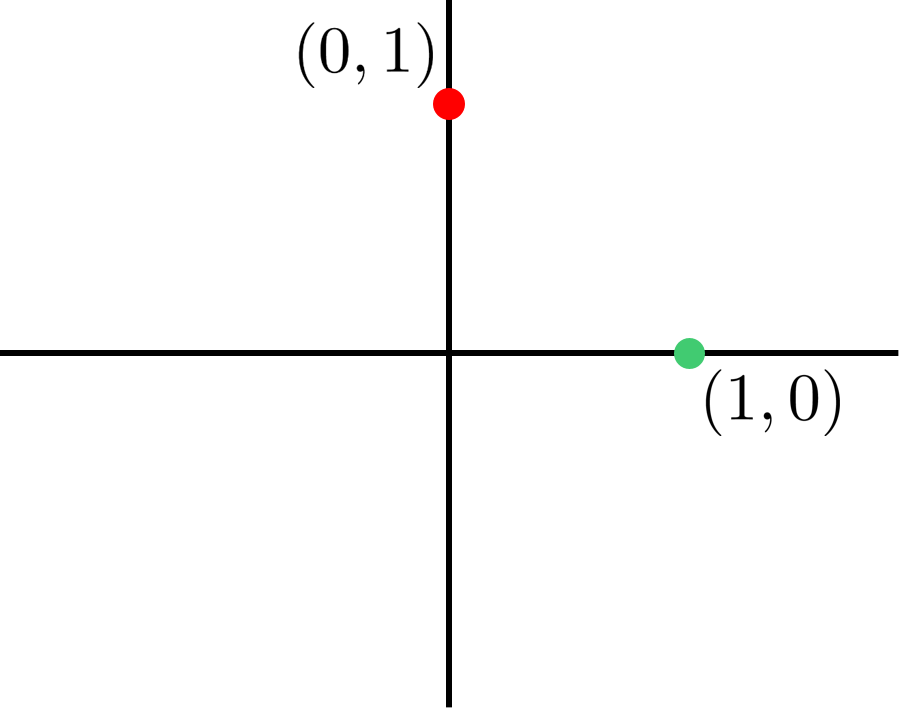
\includegraphics[width=0.4\columnwidth]{proto_blank.png}%
\hfill
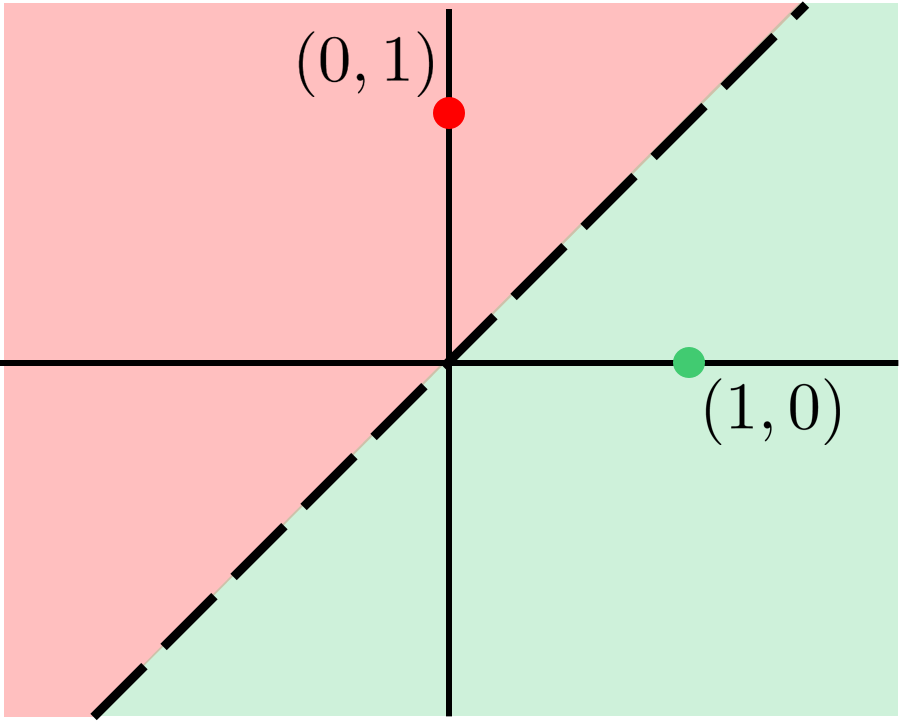
\includegraphics[width=0.4\columnwidth]{proto_euclid_sample.png}%
\caption{Learning with Prototypes: the figure on the left shows the two prototypes. The figure on the right shows what the decision boundary if the distance measure used is $d(\vz^1,\vz^2) = \norm{\vz^1-\vz^2}_2$, for any two points $\vz^1,\vz^2 \in \bR^2$. The decision boundary in this case is the line $y = x$.}%
\label{fig:proto}%
\end{figure}
\end{mlproblem}

\begin{mlproblem}[PML For Constraints]{5}
Consider the following constrained least-squares regression problem on a data set $(\vx^i,y^i)_{i=1,\ldots,n}$, where $\vx^i \in \bR^d$ and $y^i \in \bR$.
\begin{align*}
\hat\vw_\text{cls} = \arg\min&{}\ \sum_{i=1}^n(y^i - \ip{\vw}{\vx^i})^2\\
\text{s.t.}&{} \norm{\vw}_2 \leq r.
\end{align*}
Design a likelihood distribution (on the responses, conditioned on the data covariates $\vx$) and prior distribution (on the parameter) such that $\hat\vw_\text{cls}$ is the MAP estimate for your model. Give explicit forms for the density functions of your likelihood and prior distributions. The above shows that PML approaches can also lead to constrained optimization problems.
\end{mlproblem}

\begin{mlproblem}[Fun with Features]{5+5=10}
Consider the following \emph{feature-regularized} least-squares regression problem on a data set $(\vx^i,y^i)_{i=1,\ldots,n}$, where $\vx^i \in \bR^d$, $y^i \in \bR$, and $\alpha_j > 0$ for $j \in [d]$.
\[
\hat\vw_\text{fr} = \underset{\vw \in \bR^d}{\arg\min}\ \sum_{i=1}^n(y^i - \ip{\vw}{\vx^i})^2 + \sum_{j=1}^d\alpha_i(\vw_i)^2
\]
Design a likelihood and prior distribution such that $\hat\vw_\text{fr}$ is the MAP estimate for your model. Give explicit forms for all distributions. It turns out that just as there exists a closed form expression for the solution to the $L_2$-regularized least-squares problem, one exists for this problem too. Find a closed-form expression for $\hat\vw_\text{fr}$.
\end{mlproblem}

\begin{mlproblem}[Break Free from Constraints]{15}
Recall the OVA approach to multi-classification. Let us use a dataset $(\vx^i,y^i)_{i=1,\ldots,n}$, where $\vx^i \in \bR^d$ and $y^i \in [K]$ i.e. there are $K$ classes. Denote using $\vW = [\vw^1,\ldots,\vw^K] \in \bR^{d \times K}$, the set of $K$ linear models that make up the OVA classifier. The Crammer-Singer formulation $(P1)$ for a single machine learner for multi-classification is
\begin{align*}
\bc{\widehat\vW, \{\hat\xi_i\}} = \underset{\vW,\bc{\xi_i}}{\arg\min}&\ \sum_{k=1}^K\norm{\vw^k}_2^2 + \sum_{i=1}^n\xi_i\\
\text{s.t.} &\ \ip{\vw^{y^i}}{\vx^i} \geq \ip{\vw^k}{\vx^i} + 1 - \xi_i, \forall i, \forall k \neq y^i\qquad\qquad{(P1)}\\
&\ \xi_i \geq 0, \text{ for all } i
\end{align*}
Show that $(P1)$ is equivalent to the following unconstrained formulation $(P2)$
	\[
	\phantom{\hspace{20ex}}\widehat\vW = \underset{\vW}{\arg\min}\ \sum_{k=1}^K\norm{\vw^k}_2^2 + \sum_{i=1}^n\ell_\text{cs}(y^i,\veta^i)\qquad\qquad{(P2)},
	\]
	where $\veta^i = \ip{\vW}{\vx^i}$ and
	\[
	\ell_\text{cs}(y^i,\veta^i) = [1 + \max_{k \neq y}\veta^i_k - \veta^i_y]_+
	\]
	To show equivalence, you will have to show that if $\bc{\vW^0, \{\xi^0_i\}}$ are an optimum for $(P_1)$ then $\vW^0$ must be an optimum for $(P2)$, as well as if $\vW^1$ is an optimum for $(P2)$ then there must exist $\bc{\xi^1_i} \geq 0$ such that $\bc{\vW^1, \{\xi^1_i\}}$ are an optimum for $(P_1)$.
\end{mlproblem}

\begin{mlproblem}[Sub-gradient Computation]{5}
Consider the following function, where $(\vx^i,y^i)_{i=1,\ldots,n}$, where $\vx^i \in \bR^d$ and $y^i \in \bc{-1,1}$ i.e. binary Rademacher labels.
\[
f(\vw) = \sum_{i=1}^n[1 - y^i\ip{\vw}{\vx^i}]_+
\]
Suppose I construct a vector $\vg$ as follows $\vg = \sum_{i=1}^n\vh^i$, where
\[
\vh^i = \begin{cases}
-y^i\cdot\vx^i &\text{ if }\ y^i\ip{\vw}{\vx^i} < 1\\
\vzero &\text{ if }\ y^i\ip{\vw}{\vx^i} \geq 1,
\end{cases}
\]
then show that $\vg \in \partial f(\vw)$ i.e. $\vg$ is a member of the subdifferential of $f$ at $\vw$. Recall that to show this, you have to show that for every $\vw' \in \bR^d$, $f(\vw') \geq f(\vw) + \ip{\vg}{\vw'-\vw}$.
\end{mlproblem}